This chapter describes the implementation of the smartphone app and the different decisions made during this phase of the development. 
First, reasoning for the choice of target platforms is described. Then a description of the interesting parts of used libraries is provided, followed by reasoning for the choice of platform. Lastly the main design pattern is presented.

\section{Target Platform}\label{sec:targetplatform}
The first decision made, was which platforms to target. This decision has an impact on the potential user base of the app. It is not ideal if potential users are kept from using the system due to the platforms it is available on.
The two main platforms taken into consideration when choosing platform, was Android and iOS. To facilitate development for both platforms it was decided to use Xamarin \cite{xamarin} as the development platform, since Xamarin is a development platform designed with cross platform app development in mind. 

Xamarin enables reuse of significant parts of the code, thus cutting down the potential development time needed to develop for multiple platforms. Some platform specific code is still necessary for performing platform specific actions, like visual actions that is not handled through the Xamarin framework, and setting up permissions specifically for each platform. 

The individual platforms has dedicated IDE’s each (XCode \cite{xcode} for IOS, and Android Studio for Android), but none of those can facilitate the same cross platform development that Xamarin can.

The development of a full app for both platforms was however not the focus of this project, and as such development was only completed for Android as a sort of proof of concept. Additionally developing for iOS would require additional implementation: Testing if the UI works on iOS, setup of FCM on iOS, and implementation of platform specific message and notification displaying functions for iOS. The time required to develop to iOS was not available and as such, iOS version of the app was not implemented. Development was however still done using Xamarin, such that this could be done in the future.

\section{Libraries used}
The following libraries were used for the android app:
\begin{itemize}
    \item Rendy Del Rosario/FirebasePushNotificationPlugin
    \item Wilson Vargas/ButtonCircle
    \item Xamarin additional libraries
    \item dsplaisted/PCLStorage
\end{itemize}

\begin{description}
    \item [ButtonCirle] is a simple library for creating a round button.
    \item [PCLStorage] is a cross platform library for handling file IO on various mobile platforms - including Android and IOS. While an android specific library (or native android functionality) could have been used, it was decided to use PCLStorage to prepare the application for future development on a different platform.
\end{description}


\section{Server communication}
Communication with the backend part of the system is done through the API.

\begin{figure}[H]
    \centering
    \begin{lstlisting}

    HttpWebRequest request = (HttpWebRequest) HttpWebRequest.Create(url);
    request.Method = "GET";
    request.Headers.Add("email", UsernameText);
    request.Headers.Add("password", PasswordText);

    using (var response = request.GetResponse())
    {
        switch (((HttpWebResponse)response).StatusCode)
        {
            case HttpStatusCode.OK:
                using (var reader = new StreamReader(response.GetResponseStream()))
                {
                    string json = reader.ReadToEnd();
                    json = JsonConvert.DeserializeObject<dynamic>(json) ["body"].ToString();
                    currentUser = JsonConvert.DeserializeObject<User>(json);
                    currentUser.jsonCredentials = json;

                    if (currentUser.contacts == null && currentUser.id != -1)
                    {
                        CreateUserCredentialsFile(currentUser);
                        return true;
                    }

                    currentUser.setNumber();
                }
                if (currentUser.id != -1)
                {
                    CreateUserCredentialsFile(currentUser);
                    return true;
                }
                break;

            default:
                CrossPlatFormMethod.WriteTextToScreen("Kunne ikke forbinde til serveren.");
                return false;
        }
    }
\end{lstlisting}
    \caption{Login in to the server}
    \label{fig:appLogIn}
\end{figure}

Figure \ref{fig:appLogIn} is an example of the login \textit{GET} request that returns a citizen or contact. When a successful request is made, the received object is then deserialized. First, the object is converted to an object of dynamic type, containing only the body of the JSON object, since the only part of the response object of interest in is the body. The next step is then to deserialize the content of the object body into the model of a user. Separate checks are made to find out whether or not a user has a phone-number or not, and if they do, an additional deserialization is made to get the phone-number.

\section{Firebase Cloud Messaging}\label{sec:fcm}
Firebase Cloud Messaging(FCM) is used to facilitate the usage of push notifications on android. FCM works by utilizing a background service, which watches for new messages. The setup for FCM was specifically troublesome during the development. Before trying to use FCM, an attempt was made to setup an older solution from Google, Google Cloud Messaging (GCM). GCM however, proved difficult to setup. Due to this, and the amount of time that was spent on trying to make it work, it was decided to use FCM and a library instead. The library (FirebasePushNotificationPlugin by Rendy Del Rosario \cite{firebasePlugin}) ended up handling most of the setup involved in using FCM.

FCM handles user registration using tokens, which is then stored on the server-side whenever a token refresh or creation happens.

\section{Cross Platform}\label{sec:crossplat}
It was chosen to use Xamarin since this allowed for easier creation of the app for both android and IOS. But, even though Xamarin allows for code reuse between platforms, platform specific code is still necessary in some cases. This is done through a class developed specifically for this purpose for this project, namely \textit{CrossPlatformMethod}, which contains a set of static methods allowing for executing certain actions without having to consider how to do it on each platform, thus making it cross-platform. Each method then implements a version of the code that is compiled down to each platform. In this case, only the Android part is actually implemented, since that is the only platform that was developed for in this project. 

\begin{figure}[h]
    \centering
    \begin{lstlisting}
    public static void WriteTextToScreen(string message)
    {
        #if __ANDROID__
            Toast.MakeText(Xamarin.Forms.Forms.Context, message, ToastLength.Long).Show();
        #elif IOS
        #endif
    }
    \end{lstlisting}
    \caption{Multi pathform code}
    \label{fig:appMultiPlatform}
\end{figure}

Figure \ref{fig:appMultiPlatform} shows how directives is used to tell the compiler which part of the code it should compile to the different platforms. As mentioned, due to the limited scope of this project, with little focus on the app itself, this is only implemented for Android, but having methods like \ref{fig:appMultiPlatform} makes it easier to implement an iOS app in the future.

\section{MVVM Pattern}
In the app, the MVVM( Model View ViewModel) pattern is used, to facilitate separation of the views (UI) design and viewmodels(code-behind). This makes it easier to maintain and change things down the line. It also enables development on views and viewmodels concurrently, and therefore speeds up the development process. These elements (models, views and viewmodels) are created such that they can be reused for all platforms. The usage of MVVM does have some side effects, as it has forced a different handling of views from what is normally done on Android. One specific example is that the back button on an android phone does not work when trying to navigate between the different screens. This is due to the fact that in native android views are normally separate activities, which is normally handled by having the view activities on a stack. Normally when pressing the back button the app would then kill off the topmost view, to go back to the previous one. But since no stack is used in this implementation, this does not work.

\section{Conclusion}
The app has been implemented to a working condition, with the exception of the fall-detection service.

\begin{figure}[ht]
    \centering
    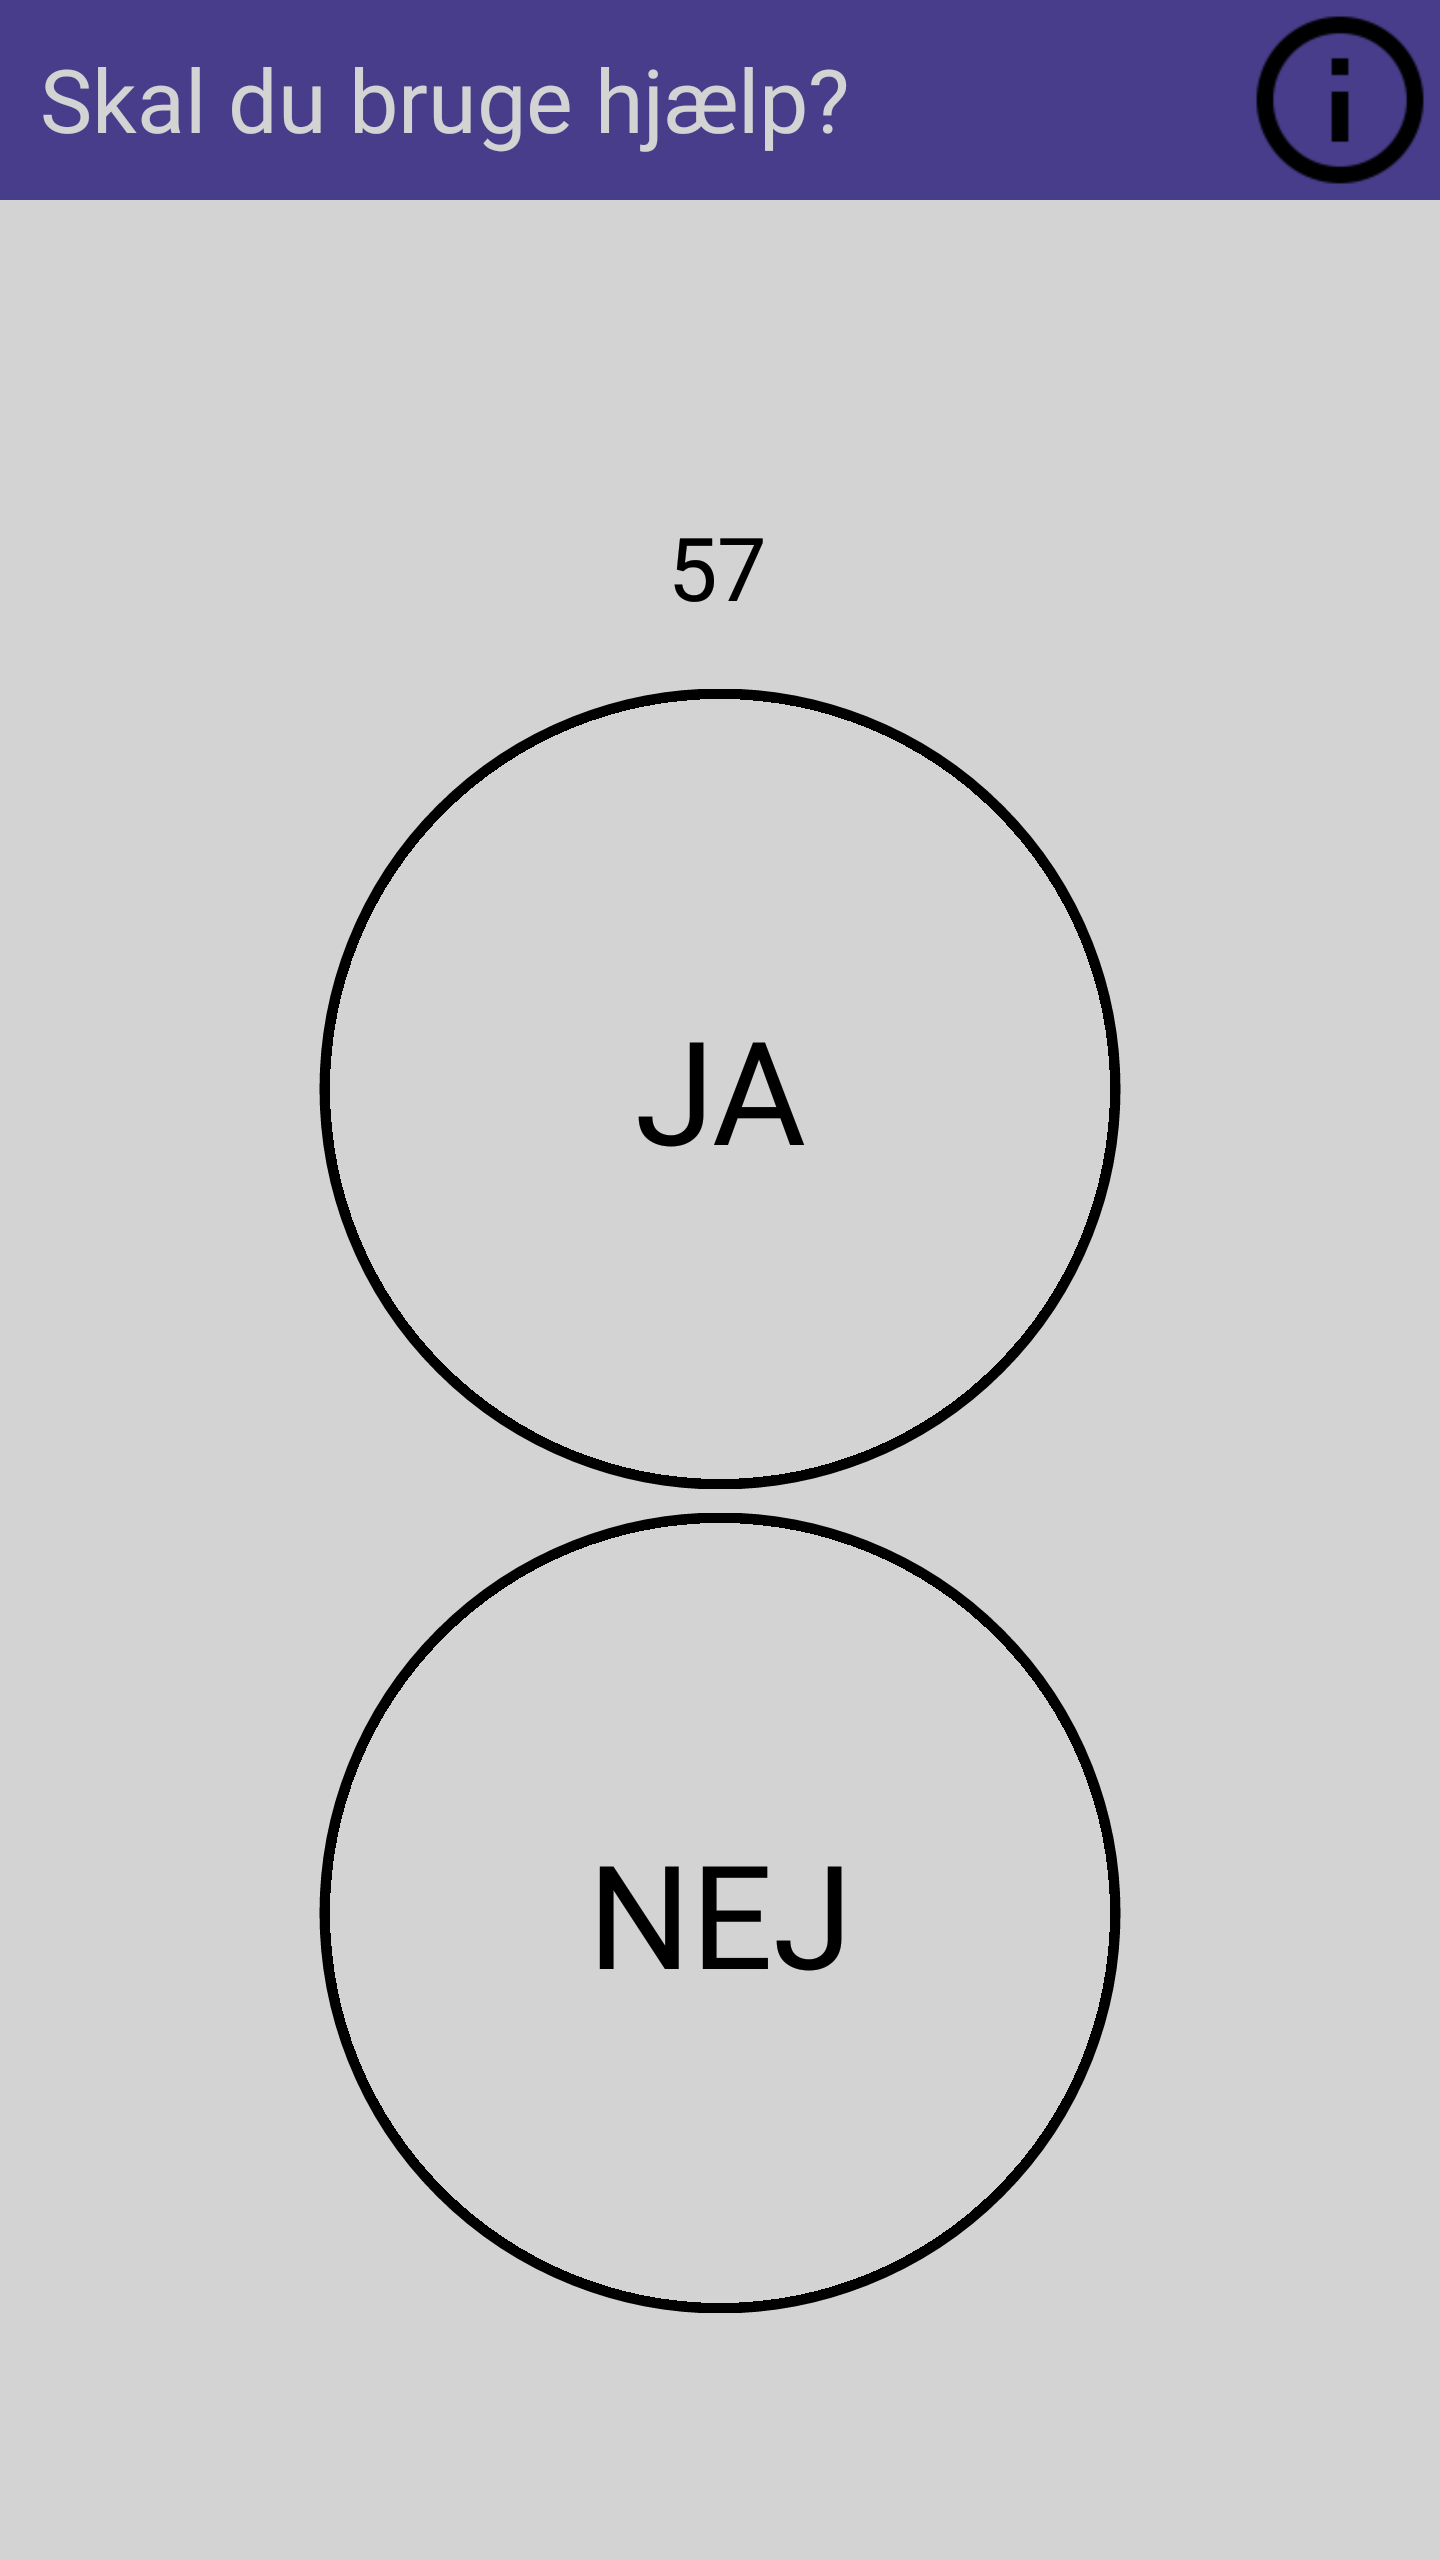
\includegraphics[scale=0.1]{Figures/usabapp.png}
    \caption{Confirmation side}
    \label{fig:usabapp}
\end{figure}

Figure \ref{fig:usabapp} shows a screenshot of the view, where a citizen confirms whether or not they need help.

\todo{Tilføj flere billeder og beskriv dem}